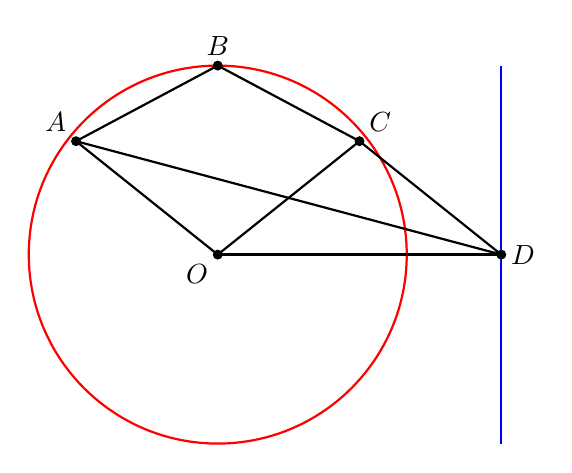
\begin{tikzpicture}[scale=1.2]
  % Circle center O and radius
  \coordinate (O) at (0,0);
  \def\r{2}

  % Circle
  \draw[red, thick] (O) circle (\r);

  % Points on/around circle (adjust as needed)
  \coordinate (A) at (-1.5,1.2);
  \coordinate (B) at (0,\r);        % top point on circle
  \coordinate (C) at (1.5,1.2);

  % Vertical line with point D to the right
  \draw[blue, thick] (3,-2) -- (3,2);
  \coordinate (D) at (3,0);

  % Quadrilateral OABC
  \draw[thick] (O) -- (A) -- (B) -- (C) -- cycle;

  % Connection to D (diamond-like shape)
  \draw[thick] (A) -- (D) -- (C);
  \draw[thick] (O) -- (D);

  % Tangent-like segments from O to A,B,C (optional emphasis)
  % (Already drawn as part of quadrilateral, but you can style them)
  % \draw[thick] (O) -- (A);
  % \draw[thick] (O) -- (B);
  % \draw[thick] (O) -- (C);

  % Mark points
  \fill (O) circle (1.5pt);
  \fill (A) circle (1.5pt);
  \fill (B) circle (1.5pt);
  \fill (C) circle (1.5pt);
  \fill (D) circle (1.5pt);

  % Labels
  \node[below left]  at (O) {$O$};
  \node[above left]  at (A) {$A$};
  \node[above]       at (B) {$B$};
  \node[above right] at (C) {$C$};
  \node[right]       at (D) {$D$};
\end{tikzpicture}
